\documentclass[a4paper,10pt]{article}
%\documentclass[a4paper,10pt]{scrartcl}

\usepackage[utf8]{inputenc}

% ------
% Clickable URLs
\usepackage{hyperref}
\usepackage{fullpage}
\usepackage{graphicx}
\usepackage[rightcaption]{sidecap}
\usepackage{microtype}
\usepackage{wrapfig}


\title{PhoneX system \\ (confidential, subject to NDA)}
\author{Du\v{s}an Klinec}
\date{}

\pdfinfo{%
  /Title    (PhoneX system)
  /Author   (Du\v{s}an Klinec)
  /Creator  (Du\v{s}an Klinec)
  /Producer ()
  /Subject  ()
  /Keywords ()
}


\begin{document}
\maketitle

\section{Product outline}
\begin{itemize}
 \item PhoneX is a solution for a secure mobile communication.
 \item Currently we support secure voice calls, text messages and a file transfer among users in the PhoneX system.
 \item PhoneX system is designed as a closed system in a sense that only PhoneX users can talk securely to each other. Main reason is the security. We set high security level
and it can be guaranteed only inside our system.
 \item Encryption is performed directly on end devices, PhoneX is an end-to-end encryption system. Server, administrators and arbitrary third parties are not 
able to eavesdrop user's communication.
 \item Voice call is transmitted over a data channel, no SIM card is required.
 \item Our voice call has low bandwidth requirements. One way (half-duplex) data channel requires 8--20 kbits per second.
\end{itemize}

\paragraph{Available platforms}
\begin{itemize}
 \item Android platform fully supported, available on Google Play.
 \item iOS platform in development. Complete client scheduled by the end of 2014.
 \item Desktop platforms scheduled to Q1,Q2/2015.
\end{itemize}

\section{System architecture}
This section briefly describes overall PhoneX architecture. Some aspects are simplified for easy understanding.
\begin{itemize}
 \item PhoneX system consists of a PhoneX cluster and PhoneX client application. Figure \ref{fig:diag_architecture} displays basic PhoneX system architecture.
 \item One PhoneX license corresponds to one user identity, identified by it's login name. User identity is explained more in section \ref{sec:identity}. 
 \item Each identity has assigned a home PhoneX cluster. This cluster manages particular user identity and it's contact list. Home cluster has minimal
information about identities (e.g., no logs are stored, messages are kept in end devices, private key is unknown to the server).
 \item Identities can communicate between each other, even if they both reside on a different PhoneX cluster. 
\end{itemize}

\begin{center}
\begin{figure}[h!]
\centering
{\scalebox{0.70}{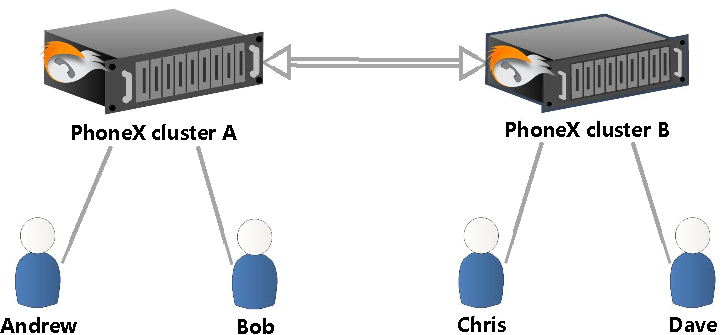
\includegraphics[trim=0 0 0 0]{phonex_architecture-crop.pdf}}}
\caption{PhoneX system architecture.}
\label{fig:diag_architecture}
\end{figure}
\end{center}


\section{User identity}\label{sec:identity}
This section describes how the user is represented in the PhoneX.
\begin{itemize}
 \item Each user represents a single identity in the system. E.g., user Alpha, identified by it's resource identifier (like mail address) and service password. Example:
\begin{itemize}
 \item \verb|alpha@phone-x.net|
 \item \verb|password123456|
\end{itemize}
 \item Each user can use PhoneX system on multiple devices. E.g., device A, device B.\footnote{Not implemented yet.} Example:
\begin{itemize}
 \item \verb|alpha@phone-x.net/deviceA|
 \item \verb|alpha@phone-x.net/deviceB|
\end{itemize}
 \item Each device user Alpha uses, generates own asymmetric key-pair. 
\begin{itemize}
 \item Currently: RSA 2048 bits.
 \item Private key never leaves the device.
 \item Private key is stored in a secure way on the device (strong encryption).
 \item Next plans: 4096, elliptic curves.
\end{itemize}
 \item \emph{X509v3 Certificate}, binding user identity and his public key is generated by the server during the first login. Home PhoneX cluster is a certification 
authority for the identity.
\begin{itemize}
 \item Certificate is stored on the user's device.
 \item This client certificate is used for authentication to PhoneX servers, in \emph{TLS} connections.
 \item PhoneX uses this certificate for digital signatures verification.
\end{itemize}
\end{itemize}


% \begin{wrapfigure}{r}{0.5\textwidth}
\begin{center}
\begin{figure}[h!]
\centering
{\scalebox{0.70}{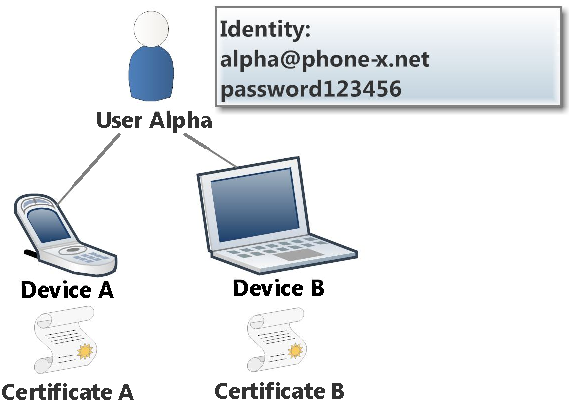
\includegraphics[trim=0 0 0 0]{user_identity-crop.pdf}}}
\caption{User identity scheme.}
\label{fig:identity}
\end{figure}
\end{center}

\subsection{Password bruteforce protection}
\begin{itemize}
 \item User's password is kept secret, only user knows it. It is unknown to server, administrators and anybody else in a plaintext form. 
 \item PhoneX mitigates weak user passwords problem by using strong password derivation functions.
 \item From the user password, several cryptographically independent secure passwords are generated using state-of-the art key derivation algorithms:
\begin{itemize}
 \item Scrypt\footnote{Protects \url{https://litecoin.org/} crypto currency. Designed to resist hardware crackers.}
 \item PBKDF2, 8192 iterations, SHA-256 HMAC mode.
\end{itemize}
 \item Dictionary/bruteforce password cracking of our password scheme is very slow, 
\begin{itemize}
 \item 16 passwords per second on 1.8 GHz, iCore 5.
 \item 0.3 passwords per second on iPhone 4.
\end{itemize}
\end{itemize}

\paragraph{Protection extension}
\begin{itemize}
 \item We have designed a new password scheme protocol that provides total protection against password bruteforcing.
 \item It works as a PIN code with ATM card, several attempts are allowed, then timeout increases. 
 \item After too many attempts, CAPTCHA solving is required.
 \item Server interaction is required, password cannot be cracked offline, server limits login attempts.
 \item Implementation of this feature scheduled to Q1/2015.
\end{itemize}

\subsection{Secure storage}
\begin{itemize}
 \item Private key is stored in an encrypted container \emph{PKCS12}, protected by a strong encryption password derived from the user password.
 \item User's private data, (e.g., contacts, messages, call logs) are stored in encrypted \emph{SQLCipher}\footnote{\url{https://www.zetetic.net/sqlcipher/}} database.
\begin{itemize}
 \item SQLCipher is an open source extension to SQLite that provides transparent 256-bit AES encryption of database files.
\end{itemize}
 \item In case of a theft or a device loss, data is protected in an encrypted form. It cannot be read without user password.
\end{itemize}

\subsection{Client communication}
\begin{itemize}
 \item PhoneX clients do not communicate directly (in a P2P manner) by default but through their home PhoneX servers.
\begin{itemize}
 \item Only exception for direct communication is during voice call, if system manages to establish a direct connection between users.
\end{itemize}
 \item Communication with the PhoneX clusters is protected by \emph{TLS} protocol, using both server and client certificate verification. 
\end{itemize}

\subsection{Contact list}
\begin{itemize}
 \item Each identity defines it's own \emph{contact list}. It is a list of identities that are allowed to contact list owner. 
 \item Contact list establishes an asymmetric trust relation. By adding user B to my contact list I allow user B to contact me
and I express my intention in receiving B's presence updates.
\begin{itemize}
 \item Users can add arbitrary users to their's contact lists.
 \item In order to communicate A and B with each other they have to at first add each other to their contact lists.
\end{itemize}
 \item Example contact list is shown in figure \ref{fig:contactlist}.
 \item Contact list is stored on the server so it can block incoming requests that are not authorized.  
 \item Contact list contains public certificate for each user so user can verify digital signatures produced by contacts and/or use it for asymmetric encryption.
 \item Contact list is managed by users via PhoneX application. In a corporate setup, the central administration control 
panel is planned on Q1/2014. The control panel will have the following features:
\begin{itemize}
 \item Centralized user management.
 \item Centralized policy management for users.
 \item Definition of user groups, levels and privileges.
 \item Integration with customer's user database.
\end{itemize}
\end{itemize}


\begin{center}
\begin{figure}[h!]
\centering
{\scalebox{0.70}{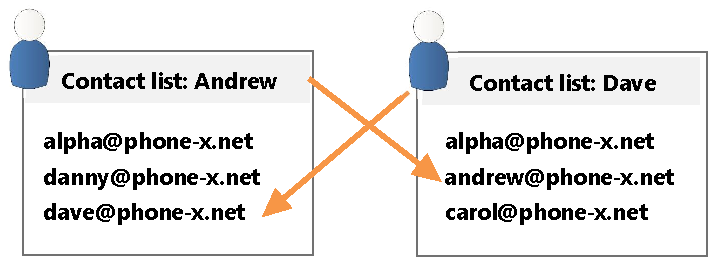
\includegraphics[trim=0 0 0 0]{contactlist-crop.pdf}}}
\caption{Example contact list for two users.}
\label{fig:contactlist}
\end{figure}
\end{center}
% \end{wrapfigure}

\subsection{Presence}
\begin{itemize}
 \item Each user can define it's own presence, displayed to other PhoneX users. Typical presence statuses are: Online, Away, Invisible.
 \item Presence is based on \emph{XMPP}. 
 \item Presence updates are sent from user to home PhoneX cluster. Then, PhoneX cluster pushes presence updates to all subscribed users.
 \item Presence information conveys additional information about the user (e.g., his certificate version, capabilities of the client / supported features.) so subscribers can react on 
changes and choose the best protocol for communication.
 \item Presence updates from A to B are sent only if A has B in the contact list and vice versa.
\end{itemize}

\section{Voice call}
\begin{itemize}
 \item \emph{SIP} is used for signaling (i.e., initiating a voice call / multimedia session among PhoneX users).
 \item \emph{ZRTP} is used to establish a shared symmetric encryption keys prior voice call. 
 \item \emph{SRTP} is used to protect a multimedia session between users by a symmetric cipher, using password derived by ZRTP.
 \item SIP packets are digitally signed so they cannot be forged by attackers. The authenticity of the requests is guaranteed.
\end{itemize}
 
\subsection{ZRTP}
\begin{itemize}
 \item An unique encryption key is established for each voice call.
 \item Encryption keys are destroyed right after finishing voice call.
 \item ZRTP internally uses \emph{Diffie-Hellman} key establishment protocol.
 \item Perfect forward secrecy property. I.e., even if long term secret is compromised (i.e., private key), the past voice call session recorded by an eavesdropper cannot be decrypted.
 \item ZRTP is protected against man-in-the-middle attacks by \emph{SAS} hash. SAS has to be verified verbally by both sides during the first voice call. After this verification
it is no more required since shared secrets from past are used to protect further communication from attackers. Example of the SAS verification dialog is depicted in figure \ref{fig:sas}.
 \item ZRTP negotiation happens in the RTP media channel, it can happen directly between users, without server interaction. It is a different flow from SIP signaling that uses server.
 \item Added value: Another layer of man-in-the-middle attack protection is employed. \emph{ZRTP hash} sent by the SIP layer is digitally signed. If the signature matches, it is guaranteed there
is no man-in-the-middle attacker in the session.
\end{itemize}

\begin{center}
\begin{figure}[h!]
\centering
{\scalebox{0.25}{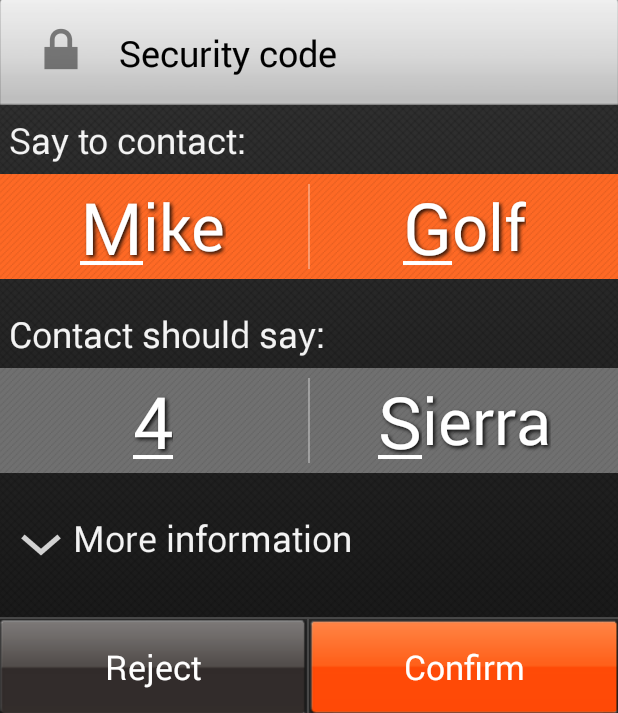
\includegraphics[trim=0 0 0 0]{sas.png}}}
\caption{SAS verification dialog.}
\label{fig:sas}
\end{figure}
\end{center}

\subsection{Call establishment}
\begin{itemize}
 \item Assume A wants to call B.
 \item A starts SIP INVITE session with B according to SIP protocol, using it's home PhoneX cluster.
 \item Call session is forbidden if they to not have each other in their contact lists.
 \item \emph{ICE}, \emph{STUN} and \emph{TURN} protocols are used to establish a direct connection between A and B.
\begin{itemize}
 \item Server does not have to forward encrypted communication between parties.
 \item Better server infrastructure scalability. 
 \item No direct bottleneck for multimedia sessions.
 \item Connection usually has better parameters (e.g., jitter, latency).
 \item Added security benefits -- no central forwarding element, DoS protection.
 \item Added value: We designed and published a new tunneling protocol for a symmetric NAT. 
This improves success ratio of establishing a direct connection between users.
 \item System has a fallback option, if direct connection cannot be established due to strict firewall settings. Relay servers are used in this case.
 \item Relay servers have small code and memory footprint, they can be deployed to the cloud to improve PhoneX system scalability.
\end{itemize}
 \item ZRTP establishes a shared symmetric encryption key over negotiated media channel.
 \item SRTP uses symmetric encryption to protect transmitted voice data, using key derived by ZRTP.
\end{itemize}

\begin{center}
\begin{figure}[h!]
\centering
{\scalebox{0.7}{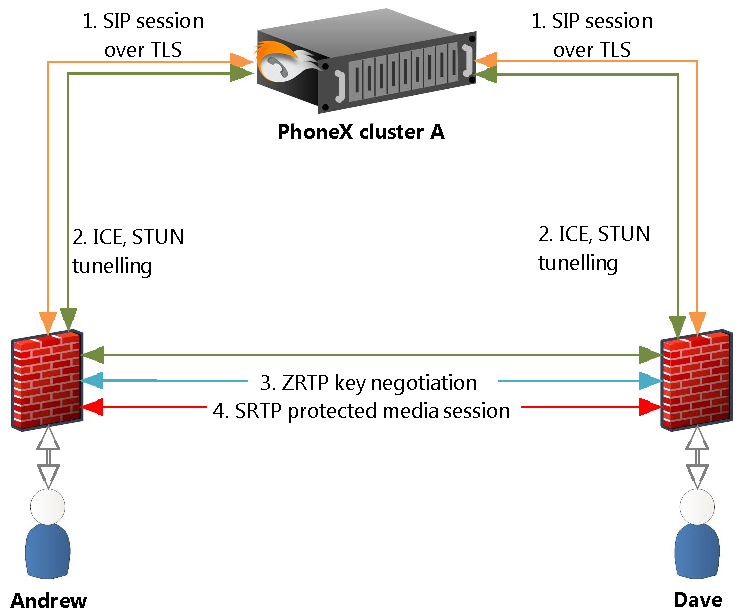
\includegraphics[trim=0 0 0 0]{phonex_call_setup-crop.pdf}}}
\caption{Simplified call setup.}
\label{fig:call}
\end{figure}
\end{center}

\subsection{Conference call}
\begin{itemize}
 \item This feature is planned on Q2/2015. 
 \item Multiple modes of operations are designed.
\end{itemize}

\section{Text messages}
\begin{itemize}
 \item Text messages work very similar to PGP. End-to-end encryption is used. Server does not see message content.
 \item Messages are encrypted using asymmetric public key of a recipient. Hybrid encryption with \emph{AES-256-GCM} is used.
 \item Text messages are delivered by SIP protocol. It enables delivery acknowledgements and offline messages.
 \item Offline messages are stored on server and forwarded to the user when he is connected again.
 \item Message read notification (i.e., message was really seen by user in the PhoneX application) are currently being tested and will be released in a next version.
 \item We designed a highly flexible messaging protocol that enables us to change encryption scheme of the messages in future releases 
to protocols with better properties.
\end{itemize}

\section{File transfer}
\begin{itemize}
 \item File transfer protocol enables secure asynchronous file transfer between PhoneX users using strong end-to-end encryption.
 \item Arbitrary files can be sent between users (images, music, binary data).
 \item Our protocol has perfect forward secrecy property. For each file, a new unique encryption 
password is derived with contribution of both parties.
\end{itemize}

\subsection{Basic principle}
\begin{itemize}
 \item For each user in the contact list PhoneX client generates \emph{N} \emph{half-keys} and stores them on the server.
 \item These half-keys can be seen as an \emph{open file slots}, that we provide for given users. I.e., 
if we generate 5 half-keys for user Andrew, then Andrew can send us 5 files and no more. % Moreover, another user, for instance Dave cannot use  Andrew's keys to send us a file since they are not valid for him.
 \item This system design has a very good anti-SPAM and anti-DoS properties since we generate half-keys only for the contacts we wish to receive files from.
 \item System is highly flexible. Number of generated half-keys can vary from contact to contact, depending on the current needs.
 \item Protocol works in an asynchronous manner. Contacts does not have to be online at the same time in order to perform file transfer.
\end{itemize}

\paragraph{Setup}
\begin{itemize}
 \item In the initialization phase, half-keys are generated for each user in the contact list and stored on the home PhoneX cluster.
 \item Keys are generated in such a way, that only a recipient can understand them, nobody else (e.g., server, administrators, other users) can understand the half-key. 
This makes our scheme resistant to a server compromise.
 \item Figure \ref{fig:ft_setup} depicts setup phase for a file transfer.
\end{itemize}

\begin{center}
\begin{figure}[h!]
\centering
{\scalebox{0.7}{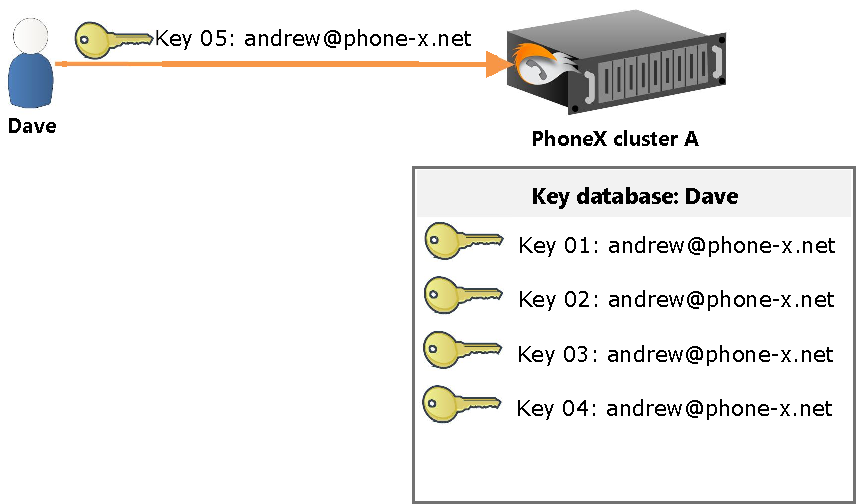
\includegraphics[trim=0 0 0 0]{phonex_filetransfer_setup-crop.pdf}}}
\caption{File transfer, key setup phase.}
\label{fig:ft_setup}
\end{figure}
\end{center}


\paragraph{Transfer}
\begin{itemize}
 \item A wants to send a file to B.
 \item A fetches half-key from the B's server, generated by B and stored for A.
 \item A generates a full key using half-key.
 \item A encrypts a file with a strong encryption and uploads this file to the server.
 \item Server stores file for later download. It does not know encryption password.
 \item Later, when B connects to the PhoneX cluster, he is notified about a new file.
 \item B downloads encrypted file from the server.
 \item B generates full encryption key for the file, verifies file authenticity and decrypts the file.
 \item Figure \ref{fig:ft_transfer} depicts file transfer protocol. 
\end{itemize}

\begin{center}
\begin{figure}[h!]
\centering
{\scalebox{0.7}{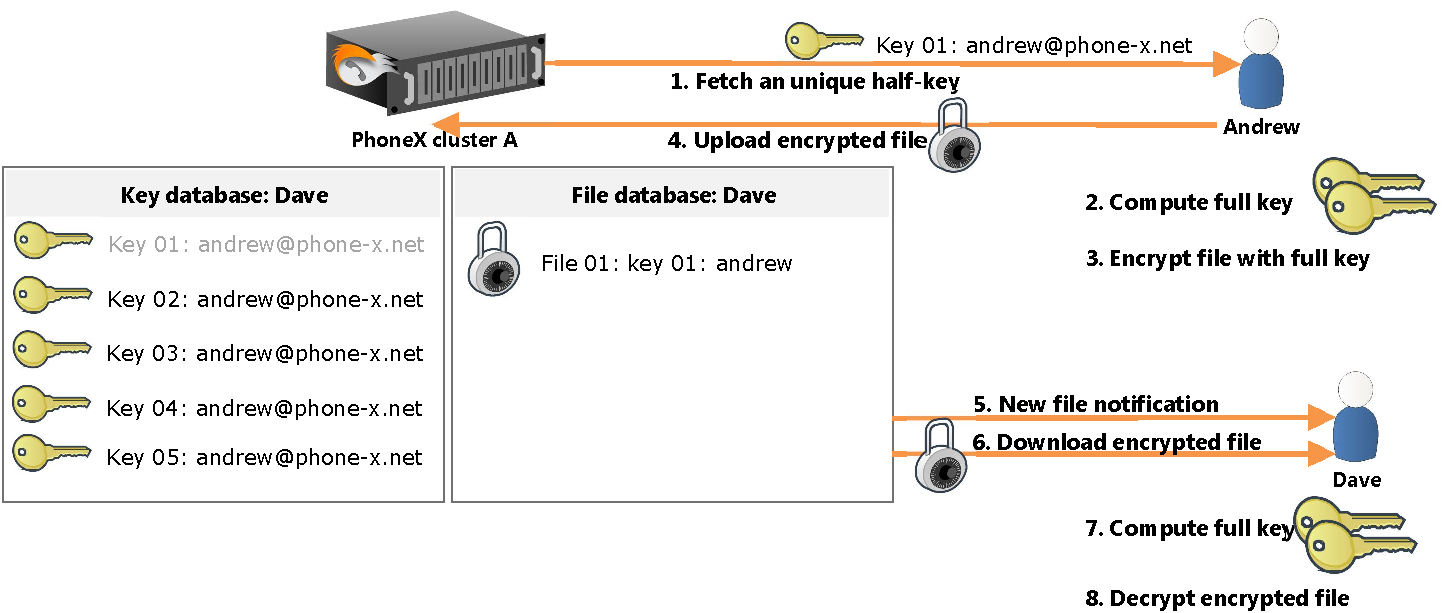
\includegraphics[trim=0 0 0 0]{phonex_filetransfer_transfer-crop.pdf}}}
\caption{File transfer.}
\label{fig:ft_transfer}
\end{figure}
\end{center}

\section{Further extensions}
We prepare more extensions to our PhoneX system, targeted on a corporate customer. Here is the example of a few:
\begin{itemize}
 \item Centralized corporate administration panel for PhoneX administration.
 \item Advanced server monitoring and usage statistics.
 \item Use of hardware security modules for increasing a security level against attackers. 
 \item Secure web client.
 \item Sending of a voice messages via file transfer, in case of poor internet connection for voice call.
 \item QR codes business cards for PhoneX system.
 \item Integration with other IM/VoIP platforms.
 \item Identity aliasing. E.g., support@phone-x.net would be redirected to currently available identity in the network.
 \item Conference calls, messages.
\end{itemize}


\end{document}
